\documentclass{article}
\usepackage[left=40mm, right=40mm, top=30mm, bottom=30mm]{geometry}
\usepackage[utf8]{inputenc}
\usepackage[italian]{babel}
\usepackage{amssymb}
\usepackage{amsthm}
\usepackage{graphics}
\usepackage{amsfonts}
\usepackage{listings}
\usepackage{amsmath}
\usepackage{amstext}
\usepackage{engrec}
\usepackage{rotating}
\usepackage{verbatim}
\usepackage[safe,extra]{tipa}
\usepackage{multirow}
\usepackage{hyperref}
\usepackage{microtype}
\usepackage{enumerate}
\usepackage{physics}
\usepackage{braket}
\usepackage{multicol}
%\usepackage{mhchem}
\usepackage{marginnote}
%\usepackage{pgfplots}
\usepackage{cancel}
\usepackage{polynom}
\usepackage{booktabs}
\usepackage{enumitem}
\usepackage{framed}
\usepackage{pdfpages}
\usepackage{algorithm}
% \usepackage{algpseudocode}
\usepackage[cache=false]{minted}
\usepackage{mathtools}
\usepackage[noend]{algpseudocode}
\title{Hands-On}
\author{Davide Cozzi, Fabio Pirovano, Viola Rillosi, Giulia Sala}
\date{20/04/2022}
\begin{document}

\maketitle

\section*{Modello 1}
\[\mathcal{S}=\{A,\,\, R_A, \,\,P_A\}\]
\textbf{Dove}:
\begin{itemize}
  \item $A$: gene $A$
  \item $R_A$: mRNA per $A$
  \item $P_A$: proteina $A$
\end{itemize}
\begin{table}[H]
  \centering
  \begin{tabular}{c|c|c|c}
    \# & \textbf{Reagenti} & \textbf{Prodotti} & \textbf{Costanti}\\
    \hline
    \hline
    $r_1$ & $A$ & $A+R_A$ & -\\
    $r_2$ & $R_A$ & $R_A+P_A$ & -\\
    $r_3$ & $R_A$ & $\emptyset$ & -\\
    $r_4$ & $P_A$ & $\emptyset$ & -\\
  \end{tabular}
\end{table}
\newpage
\section*{Modello 2}
\[\mathcal{S}=\{A,\,\, R_A,\,\, P_A,\,\, B,\,\, R_B,\,\, P_B,\,\, A\cdot
  P_B,\,\, B\cdot P_A\}\] 
\textbf{Dove}:
\begin{multicols}{2}
  \begin{itemize}
    \item $A$: gene $A$
    \item $R_A$: mRNA per $A$
    \item $P_A$: proteina $A$
    \item $B$: gene $B$
    \item $R_B$: mRNA per $B$
    \item $P_B$: proteina $B$
    \item $A\cdot P_B$: composto di $A$ e $P_B$
    \item $B\cdot P_A$: composto di $B$ e $P_A$
  \end{itemize}
\end{multicols}
\begin{table}[H]
  \centering
  \begin{tabular}{c|c|c|c}
    \# & \textbf{Reagenti} & \textbf{Prodotti} & \textbf{Costanti}\\
    \hline
    \hline
    $r_1$ & $A$ & $A+R_A$ & -\\
    $r_2$ & $B$ & $B+R_B$ & $k_1$\\
    $r_3$ & $R_A$ & $R_A+P_A$ & -\\
    $r_4$ & $R_B$ & $R_B+P_B$ & -\\
    $r_5$ & $A+P_B$ & $A\cdot P_B$ & -\\
    $r_6$ & $B+P_A$ & $B\cdot P_A$ & -\\
    $r_7$ & $B\cdot P_A$ & $R_B+B\cdot P_A$ & $k_2$\\
    $r_8$ & $A\cdot P_B$ & $A+P_B$ & -\\
    $r_9$ & $B\cdot P_A$ & $B+P_A$ & -\\
    $r_{10}$ & $R_A$ & $\emptyset$ & -\\
    $r_{11}$ & $R_B$ & $\emptyset$ & -\\
    $r_{12}$ & $P_A$ & $\emptyset$ & -\\
    $r_{13}$ & $P_B$ & $\emptyset$ & -\\
  \end{tabular}
\end{table}
\textbf{Assunzioni}:
\begin{itemize}
  \item $k_2>k_1$
\end{itemize}
\newpage
\section*{Modello 3}
\[\mathcal{S}=\{A,\,\, R_A,\,\, P_A,\,\, B,\,\, R_B,\,\, P_B,\,\,C,\,\, R_C,\,\,
  P_C,\,\, A\cdot P_B,\,\, B\cdot P_A,\,\, P_B^P,\,\, C\cdot P_B^P,\,\,  C\cdot 
  2P_B^P,\,\,  K,\,\, F\}\]    
\textbf{Dove}:
\begin{multicols}{2}
  \begin{itemize}
    \item $A$: gene $A$
    \item $R_A$: mRNA per $A$
    \item $P_A$: proteina $A$
    \item $B$: gene $B$
    \item $R_B$: mRNA per $B$
    \item $P_B$: proteina $B$
    \item $C$: gene $C$
    \item $R_C$: mRNA per $C$
    \item $P_C$: proteina $C$
    \item $A\cdot P_B$: composto di $A$ e $P_B$
    \item $B\cdot P_A$: composto di $B$ e $P_A$
    \item $P_B^P$: $P_B$ fosforilata
    \item $C\cdot P_B^P$: composto di $C$ e $P_B^P$
    \item $C\cdot 2P_B^P$: composto di $C\cdot P_B^P$ e $P_B^P$
    \item $K$: chinasi
    \item $F$: fosfatasi
  \end{itemize}
\end{multicols}
\begin{table}[H]
  \centering
  \begin{tabular}{c|c|c|c}
    \# & \textbf{Reagenti} & \textbf{Prodotti} & \textbf{Costanti}\\
    \hline
    \hline
    $r_1$ & $A$ & $A+R_A$ & -\\
    $r_2$ & $B$ & $B+R_B$ & $k_1$\\
    $r_3$ & $C$ & $C+R_C$ & $k_2$\\
    $r_4$ & $R_A$ & $R_A+P_A$ & -\\
    $r_5$ & $R_B$ & $R_B+P_B$ & -\\
    $r_6$ & $R_C$ & $R_C+P_C$ & -\\
    $r_7$ & $A+P_B$ & $A\cdot P_B$ & -\\
    $r_8$ & $B+P_A$ & $B\cdot P_A$ & -\\
    $r_9$ & $B\cdot P_A$ & $R_B+B\cdot P_A$ & $k_3$\\
    $r_{10}$ & $P_B+K$ & $P_B^P+K$ & -\\
    $r_{11}$ & $P_B^P+C$ & $C\cdot P_B^P$ & -\\
    $r_{12}$ & $C\cdot P_B^P$ & $R_C+C\cdot P_B^P$ & $k_4$\\
    $r_{13}$ & $C\cdot P_B^P+P_B^P$ & $C\cdot 2P_B^P$ & -\\
    $r_{14}$ & $C\cdot 2P_B^P$ & $C\cdot P_B^P+P_B^P$ & -\\
    $r_{15}$ & $C\cdot P_B^P$ & $P_B^P+C$ & -\\
    $r_{16}$ & $P_B^P+F$ & $P_B+F$ & -\\
    $r_{17}$ & $A\cdot P_B$ & $A+P_B$ & -\\
    $r_{18}$ & $B\cdot P_A$ & $B+P_A$ & -\\
    $r_{19}$ & $R_A$ & $\emptyset$ & -\\
    $r_{20}$ & $R_B$ & $\emptyset$ & -\\
    $r_{21}$ & $R_C$ & $\emptyset$ & -\\
    $r_{22}$ & $P_A$ & $\emptyset$ & -\\
    $r_{23}$ & $P_B$ & $\emptyset$ & -\\
    $r_{24}$ & $P_C$ & $\emptyset$ & -\\
  \end{tabular}
\end{table}
\textbf{Assunzioni}:
\begin{itemize}
  \item $k_3>k_1$
  \item $k_4<k_2$
\end{itemize}
Equazioni differenziali ottenute con COPASI (con i \textit{reaction rate} ``a
caso'' con il solo mantenimento ``a spanne'' delle due assunzioni):
\scriptsize{
  %%% Attention: 
%%% We provide only the LaTeX code of the Differential Equations. 
%%% You need to include it in your TeX document. 
%%% Some manual adjustments may be needed for too wide equations. 

$$
\begin{array}{ccl}
\frac {\mathrm{d}\left( {{\mathrm{[A]}} \, \cdot \, {V}_{\mathrm{compartment}} } \right) }  {\mathrm{d}{t} }  \; &=& \;  { \, - \, {V}_{\mathrm{compartment}} \, \cdot \, \left(\left( {{0.1} \, \cdot \, {\mathrm{[A]}} \, \cdot \, {\mathrm{[PB]}} \, - \, {0.1} \, \cdot \, {\mathrm{[APB]}} } \right)\right) } \\ 
 && \\ 
\frac {\mathrm{d}\left( {{\mathrm{[B]}} \, \cdot \, {V}_{\mathrm{compartment}} } \right) }  {\mathrm{d}{t} }  \; &=& \;  { \, - \, {V}_{\mathrm{compartment}} \, \cdot \, \left(\left( {{0.1} \, \cdot \, {\mathrm{[B]}} \, \cdot \, {\mathrm{[PA]}} \, - \, {0.1} \, \cdot \, {\mathrm{[BPA]}} } \right)\right) } \\ 
 && \\ 
\frac {\mathrm{d}\left( {{\mathrm{[RA]}} \, \cdot \, {V}_{\mathrm{compartment}} } \right) }  {\mathrm{d}{t} }  \; &=& \;  { \, + \, {V}_{\mathrm{compartment}} \, \cdot \, \left( {{0.1} \, \cdot \, {\mathrm{[A]}} } \right) } \\ 
 && \\ 
 \; && \;  { \, - \, {V}_{\mathrm{compartment}} \, \cdot \, \left( {{0.1} \, \cdot \, {\mathrm{[RA]}} } \right) } \\ 
 && \\ 
\frac {\mathrm{d}\left( {{\mathrm{[RB]}} \, \cdot \, {V}_{\mathrm{compartment}} } \right) }  {\mathrm{d}{t} }  \; &=& \;  { \, + \, {V}_{\mathrm{compartment}} \, \cdot \, \left( {{0.1} \, \cdot \, {\mathrm{[B]}} } \right) } \\ 
 && \\ 
 \; && \;  { \, - \, {V}_{\mathrm{compartment}} \, \cdot \, \left( {{0.1} \, \cdot \, {\mathrm{[RB]}} } \right) } \\ 
 && \\ 
 \; && \;  { \, + \, {V}_{\mathrm{compartment}} \, \cdot \, \left( {{0.2} \, \cdot \, {\mathrm{[BPA]}} } \right) } \\ 
 && \\ 
\frac {\mathrm{d}\left( {{\mathrm{[PA]}} \, \cdot \, {V}_{\mathrm{compartment}} } \right) }  {\mathrm{d}{t} }  \; &=& \;  { \, - \, {V}_{\mathrm{compartment}} \, \cdot \, \left( {{0.1} \, \cdot \, {\mathrm{[PA]}} } \right) } \\ 
 && \\ 
 \; && \;  { \, + \, {V}_{\mathrm{compartment}} \, \cdot \, \left( {{0.1} \, \cdot \, {\mathrm{[RA]}} } \right) } \\ 
 && \\ 
 \; && \;  { \, - \, {V}_{\mathrm{compartment}} \, \cdot \, \left(\left( {{0.1} \, \cdot \, {\mathrm{[B]}} \, \cdot \, {\mathrm{[PA]}} \, - \, {0.1} \, \cdot \, {\mathrm{[BPA]}} } \right)\right) } \\ 
 && \\ 
\frac {\mathrm{d}\left( {{\mathrm{[PB]}} \, \cdot \, {V}_{\mathrm{compartment}} } \right) }  {\mathrm{d}{t} }  \; &=& \;  { \, + \, {V}_{\mathrm{compartment}} \, \cdot \, \left( {{0.1} \, \cdot \, {\mathrm{[PBP]}} \, \cdot \, {\mathrm{[F]}} } \right) } \\ 
 && \\ 
 \; && \;  { \, - \, {V}_{\mathrm{compartment}} \, \cdot \, \left( {{0.1} \, \cdot \, {\mathrm{[PB]}} } \right) } \\ 
 && \\ 
 \; && \;  { \, + \, {V}_{\mathrm{compartment}} \, \cdot \, \left( {{0.1} \, \cdot \, {\mathrm{[RB]}} } \right) } \\ 
 && \\ 
 \; && \;  { \, - \, {V}_{\mathrm{compartment}} \, \cdot \, \left(\left( {{0.1} \, \cdot \, {\mathrm{[A]}} \, \cdot \, {\mathrm{[PB]}} \, - \, {0.1} \, \cdot \, {\mathrm{[APB]}} } \right)\right) } \\ 
 && \\ 
 \; && \;  { \, - \, {V}_{\mathrm{compartment}} \, \cdot \, \left( {{0.1} \, \cdot \, {\mathrm{[PB]}} \, \cdot \, {\mathrm{[K]}} } \right) } \\ 
 && \\ 
\frac {\mathrm{d}\left( {{\mathrm{[APB]}} \, \cdot \, {V}_{\mathrm{compartment}} } \right) }  {\mathrm{d}{t} }  \; &=& \;  { \, + \, {V}_{\mathrm{compartment}} \, \cdot \, \left(\left( {{0.1} \, \cdot \, {\mathrm{[A]}} \, \cdot \, {\mathrm{[PB]}} \, - \, {0.1} \, \cdot \, {\mathrm{[APB]}} } \right)\right) } \\ 
 && \\ 
\frac {\mathrm{d}\left( {{\mathrm{[BPA]}} \, \cdot \, {V}_{\mathrm{compartment}} } \right) }  {\mathrm{d}{t} }  \; &=& \;  { \, + \, {V}_{\mathrm{compartment}} \, \cdot \, \left(\left( {{0.1} \, \cdot \, {\mathrm{[B]}} \, \cdot \, {\mathrm{[PA]}} \, - \, {0.1} \, \cdot \, {\mathrm{[BPA]}} } \right)\right) } \\ 
 && \\ 
\frac {\mathrm{d}\left( {{\mathrm{[PBP]}} \, \cdot \, {V}_{\mathrm{compartment}} } \right) }  {\mathrm{d}{t} }  \; &=& \;  { \, - \, {V}_{\mathrm{compartment}} \, \cdot \, \left(\left( {{0.1} \, \cdot \, {\mathrm{[PBP]}} \, \cdot \, {\mathrm{[C]}} \, - \, {0.1} \, \cdot \, {\mathrm{[CPBP]}} } \right)\right) } \\ 
 && \\ 
 \; && \;  { \, - \, {V}_{\mathrm{compartment}} \, \cdot \, \left(\left( {{0.1} \, \cdot \, {\mathrm{[CPBP]}} \, \cdot \, {\mathrm{[PBP]}} \, - \, {0.1} \, \cdot \, {\mathrm{[C2PBP]}} } \right)\right) } \\ 
 && \\ 
 \; && \;  { \, - \, {V}_{\mathrm{compartment}} \, \cdot \, \left( {{0.1} \, \cdot \, {\mathrm{[PBP]}} \, \cdot \, {\mathrm{[F]}} } \right) } \\ 
 && \\ 
 \; && \;  { \, + \, {V}_{\mathrm{compartment}} \, \cdot \, \left( {{0.1} \, \cdot \, {\mathrm{[PB]}} \, \cdot \, {\mathrm{[K]}} } \right) } \\ 
 && \\ 
\frac {\mathrm{d}\left( {{\mathrm{[C]}} \, \cdot \, {V}_{\mathrm{compartment}} } \right) }  {\mathrm{d}{t} }  \; &=& \;  { \, - \, {V}_{\mathrm{compartment}} \, \cdot \, \left(\left( {{0.1} \, \cdot \, {\mathrm{[PBP]}} \, \cdot \, {\mathrm{[C]}} \, - \, {0.1} \, \cdot \, {\mathrm{[CPBP]}} } \right)\right) } \\ 
 && \\ 
\frac {\mathrm{d}\left( {{\mathrm{[RC]}} \, \cdot \, {V}_{\mathrm{compartment}} } \right) }  {\mathrm{d}{t} }  \; &=& \;  { \, + \, {V}_{\mathrm{compartment}} \, \cdot \, \left( {{0.05} \, \cdot \, {\mathrm{[CPBP]}} } \right) } \\ 
 && \\ 
 \; && \;  { \, - \, {V}_{\mathrm{compartment}} \, \cdot \, \left( {{0.1} \, \cdot \, {\mathrm{[RC]}} } \right) } \\ 
 && \\ 
 \; && \;  { \, + \, {V}_{\mathrm{compartment}} \, \cdot \, \left( {{0.1} \, \cdot \, {\mathrm{[C]}} } \right) } \\ 
 && \\ 
\frac {\mathrm{d}\left( {{\mathrm{[PC]}} \, \cdot \, {V}_{\mathrm{compartment}} } \right) }  {\mathrm{d}{t} }  \; &=& \;  { \, - \, {V}_{\mathrm{compartment}} \, \cdot \, \left( {{0.1} \, \cdot \, {\mathrm{[PC]}} } \right) } \\ 
 && \\ 
 \; && \;  { \, + \, {V}_{\mathrm{compartment}} \, \cdot \, \left( {{0.1} \, \cdot \, {\mathrm{[RC]}} } \right) } \\ 
 && \\ 
\frac {\mathrm{d}\left( {{\mathrm{[CPBP]}} \, \cdot \, {V}_{\mathrm{compartment}} } \right) }  {\mathrm{d}{t} }  \; &=& \;  { \, + \, {V}_{\mathrm{compartment}} \, \cdot \, \left(\left( {{0.1} \, \cdot \, {\mathrm{[PBP]}} \, \cdot \, {\mathrm{[C]}} \, - \, {0.1} \, \cdot \, {\mathrm{[CPBP]}} } \right)\right) } \\ 
 && \\ 
 \; && \;  { \, - \, {V}_{\mathrm{compartment}} \, \cdot \, \left(\left( {{0.1} \, \cdot \, {\mathrm{[CPBP]}} \, \cdot \, {\mathrm{[PBP]}} \, - \, {0.1} \, \cdot \, {\mathrm{[C2PBP]}} } \right)\right) } \\ 
 && \\ 
\frac {\mathrm{d}\left( {{\mathrm{[C2PBP]}} \, \cdot \, {V}_{\mathrm{compartment}} } \right) }  {\mathrm{d}{t} }  \; &=& \;  { \, + \, {V}_{\mathrm{compartment}} \, \cdot \, \left(\left( {{0.1} \, \cdot \, {\mathrm{[CPBP]}} \, \cdot \, {\mathrm{[PBP]}} \, - \, {0.1} \, \cdot \, {\mathrm{[C2PBP]}} } \right)\right) } \\ 
 && \\ 
\end{array}
$$
}
\newpage
\noindent
\begin{figure}[H]
  \centering
  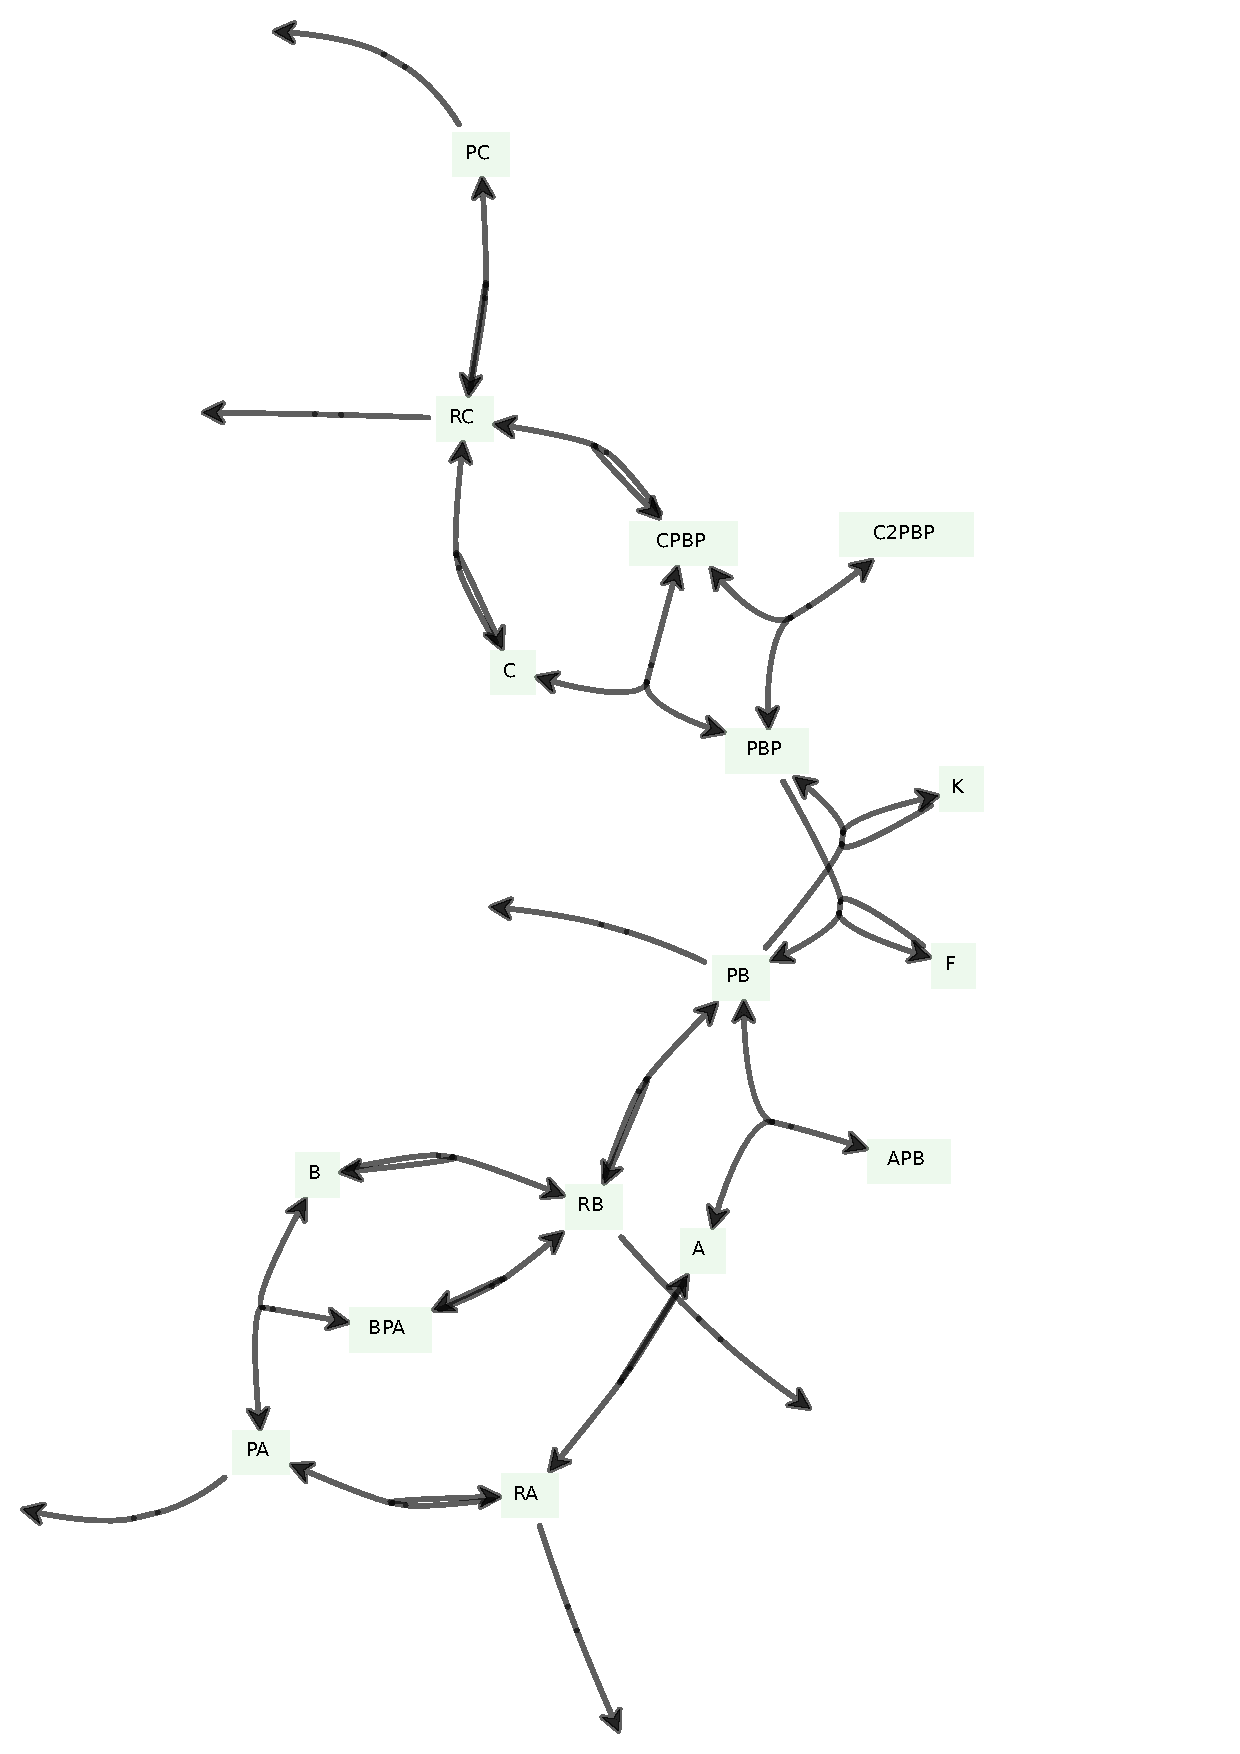
\includegraphics[width = \textwidth]{img/model.pdf}
  \caption{Modello3 rappresentato graficamente con COPASI}
  \label{fig:model3}
\end{figure}
\end{document}
